%!TEX root = ../dokumentation.tex

\section{Gestaltungslösungen}
Auf diesen Ergebnissen aufbauend, ging es in der weiteren MCI Auseinandersetzung darum, identifizierte Nutzungsanforderungen in eine Gestaltungslösung zu verarbeiten, die der Erfüllung der Anforderungen dient.
Während sich die vorherigen Prototypen durch ihren abstrakten Charakter auszeichneten und sich damit befassten "welche" Inhalte auf dem user interface zu sehen sind, so war das Ziel des nächsten Prototypen zu bestimmen, "wie" diese Inhalte auf einem user interface dargestellt werden können.\\
Das Prototyping für Designansätze liefert zudem die Möglichkeit, mit Hilfe eines realen Anwenders, Anforderungen und Gestaltungsansätze zu bewerten und vorhandene Schwachstellen aufzuweisen.\\
Zu diesem Zeitpunkt innerhalb der Projektphase, befand sich die Entwicklung bei der Implementierung der reinen Funktionalität, ohne Wert auf das Aussehen des Interface zu legen. Wie an früherer Stelle der Dokumentation bereits aufgeführt, waren einfache Mockup-Entwürfe erste Ansätze, um Struktur und Übergang der einzelnen Working Spaces zu verbessern.\\

Der Prototyp sollte den Gegebenheit des aktuellen Projektstandes entsprechen.\\ Das bedeutete:
\begin{itemize}
   \item 
 	der finanzielle Aufwand musste möglichst gering sein

   \item 
   die Entwicklung des Prototypen sollte in Anbetracht des Zeitrahmens in einer relativ kurzen Zeit geschehen

   \item 
   es sollte die Möglichkeit gegeben sein ihn leicht zu verändern

   \item
   eine Evaluation mit realen Benutzern sollte ohne technische Aufwand realisierbar sein
  
\end{itemize} 

Die Auswahl bestand auf Prototypen zweiter Kategorien,\footnote{Nach Prof. Hartmann Draft zur MCI, S.444}. papierbasierte Prototypen oder computerbasierte Prototypen. Aufgrund der benannten Bedingungen wurde die Entscheidung getroffen den Designprozess mit papierbasierten Prototypen zu beginnen, da die Entwicklung von Mockups mit Interaktionsfähigkeit oder ein codebasierter Prototyp zu viel Zeit in Anspruch genommen hätten.

\newpage
\subsection{Paperbased Prototyping}
Der Prototyp basierte auf einfachen, mit Stift und Papier entwickelten Handskizzen, wobei jedem Interface Context des zuvor entwickelten abstract prototype, ein neuer "Screen" gewidmet wurde. Durch das entworfene content model, war im Team ein deutliches Verständnis dafür, welche Inhalte vorhanden sein mussten und stellten in diesem Punkt eine Erleichertung dar. Mehrere Designsansätze wurden besprochen, wobei vorallem für die Hauptseite der Anwendung, von der aus die einzelnen Funktionalitäten aufrufbar sein sollen, unterschiedlichste Umsetzungsmöglichkeiten angedacht wurden. Eine iconbasierte Übersicht aller Funktionen, zwei verschiedene Hauptseiten, die sich per Swipe wechseln lassen und jeweils eine der primary user Rollen repräsentierten oder eine komplette anpassbare Übersicht der Funktionen. Da für die Gestaltung mehrere Iterationsphasen vorgesehen waren, fiel die Entscheidung auf den kleinsten gemeinsamen Nenner, einer listenartigen Darstellung der vorhandenen Funktionen.\\ 
Das Ziel des ersten Prototypen war es, das angedachte System erstmals zu evaluieren und dabei den Fokus auf eine optimale Navigation innerhalb der Anwendung zu legen. Für dynamische Inhalte wurden einzelne Handskizzen bei entsprechender Aktion übereinander gelegt und sollten damit die Systemreaktion für den User verdeutlichen. 
Die folgende Abbildungen in \ref{proto}, zeigen beispielhaft wie diese Interfaceseiten während des Testens aussahen. Um einen weiteren Eindruck zu erhalten, befindet sich im Anhang (Seite TODO) ein Teil des ersten Prototypsets.

\begin{figure}[H]
\centering
\hfill
\subfloat[Neue Mietanfrage anzeigen\label{pic:neueMietanfrage}]{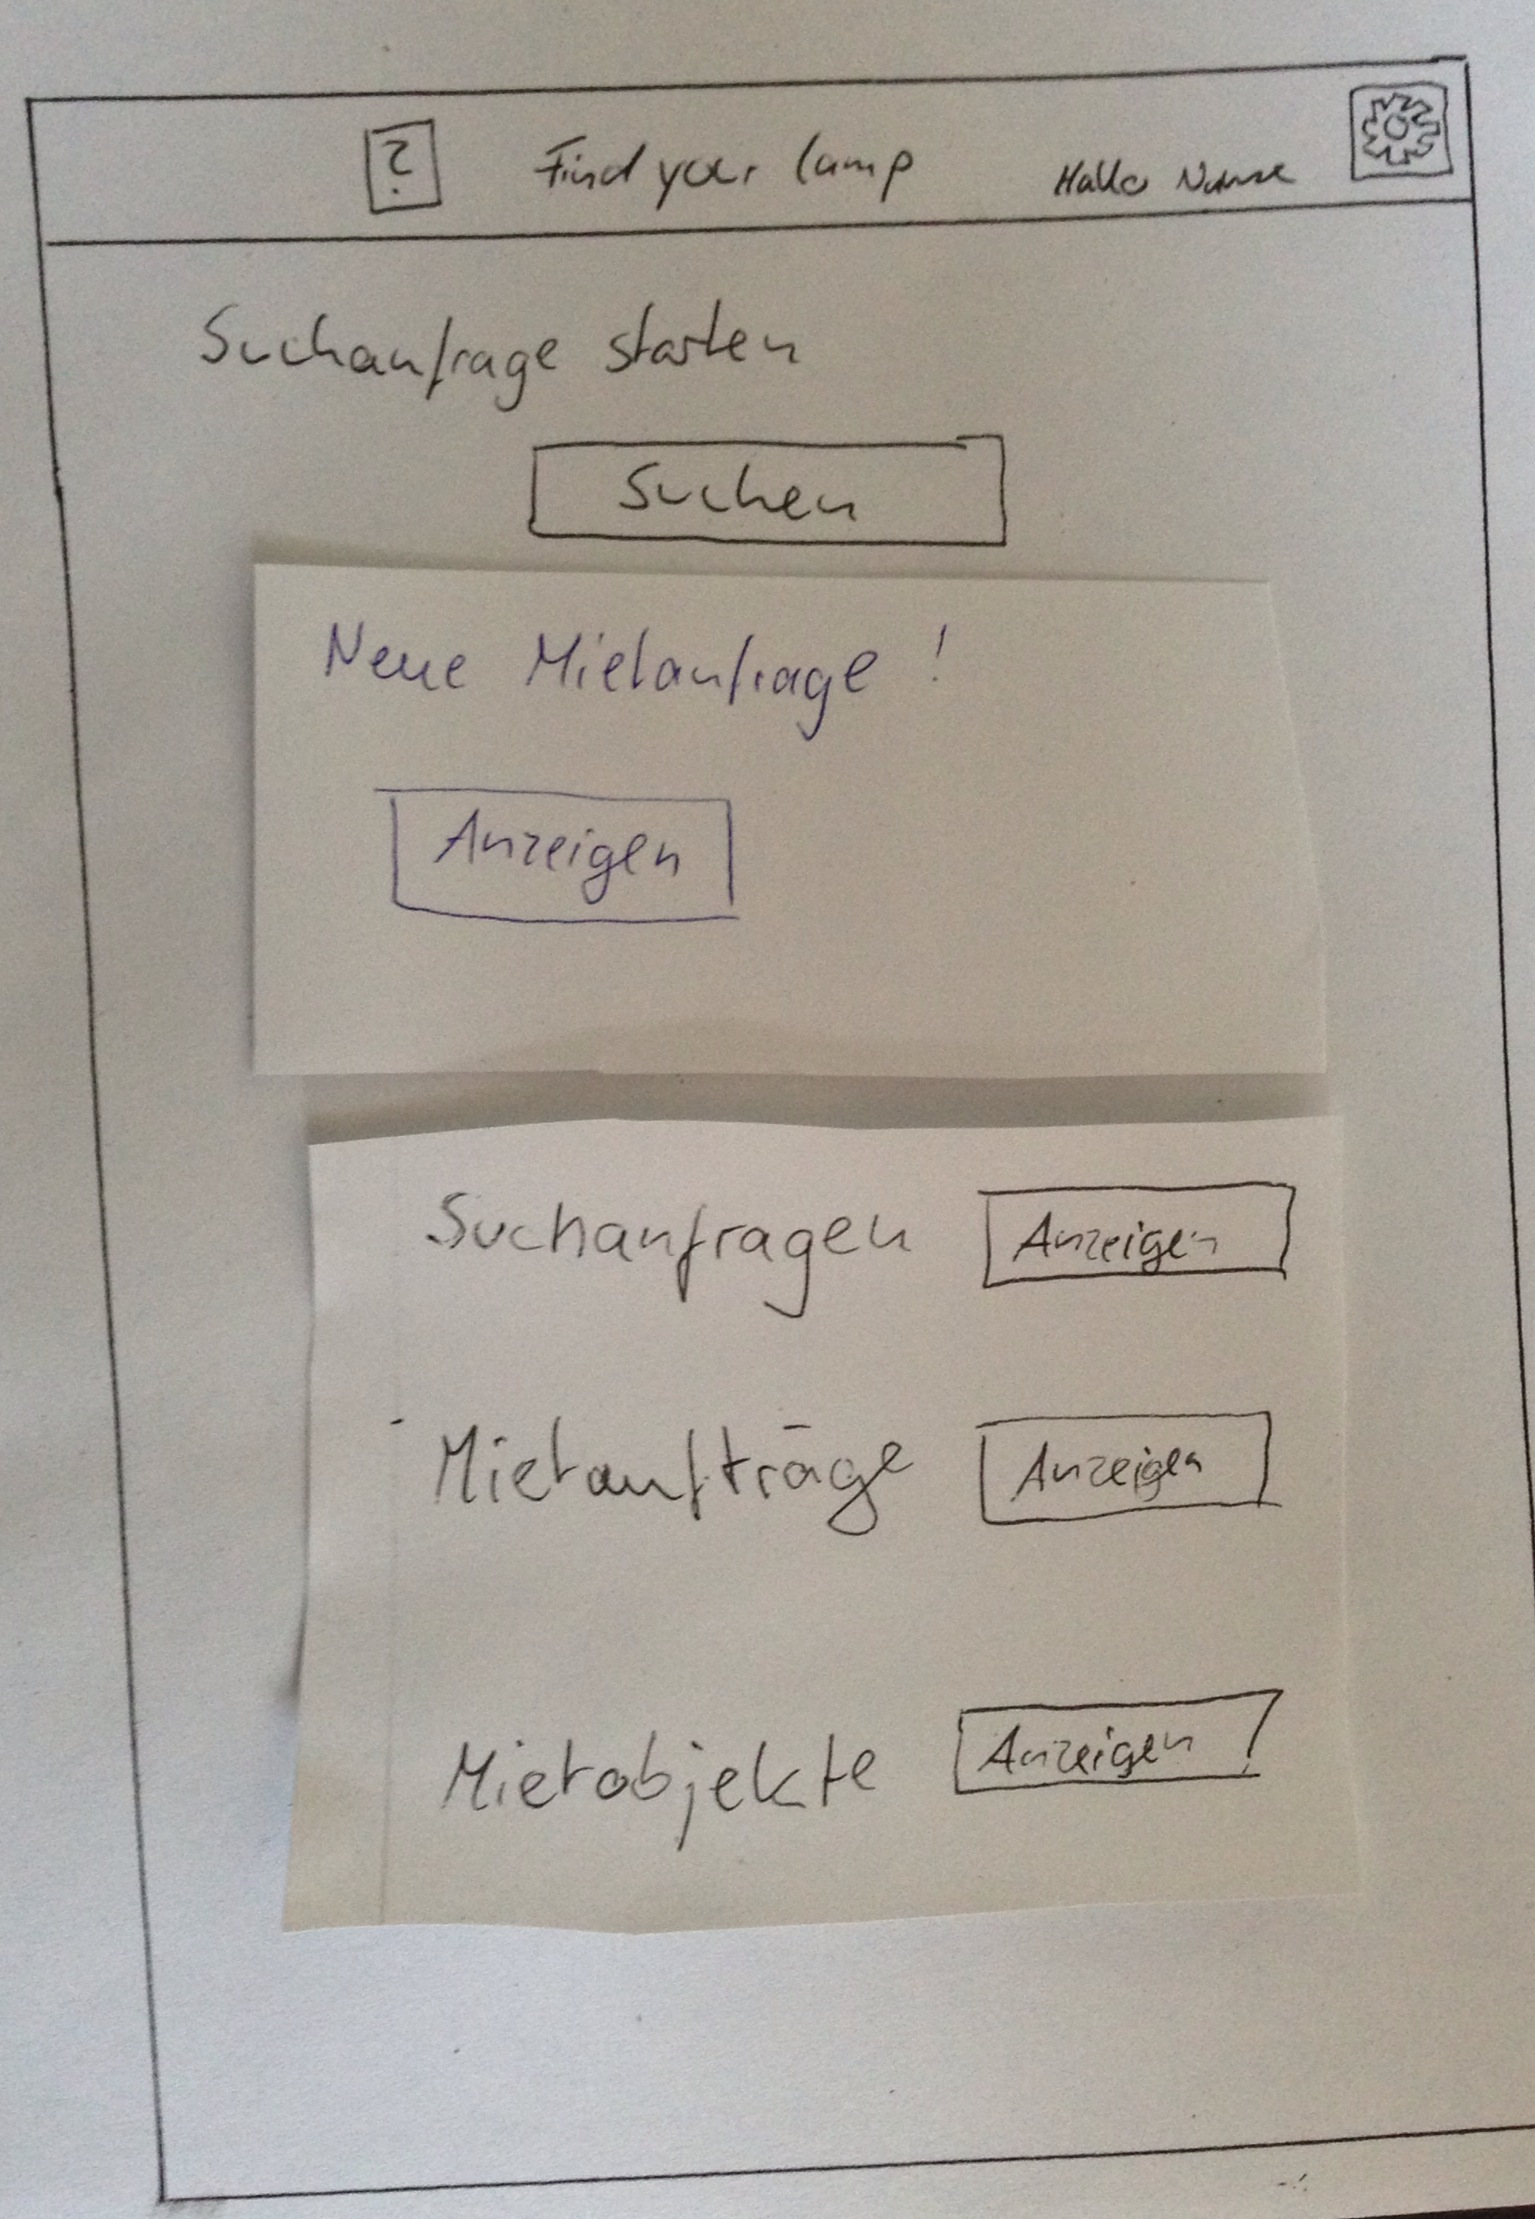
\includegraphics[width=.42\textwidth]{./images/paperbased/neueMietanfrage.JPG}}
\hfill % alternativ auch \hspace{1cm} für genaue Angaben
\subfloat[Übersicht der Suchanfragen \label{pic:anfrage}]{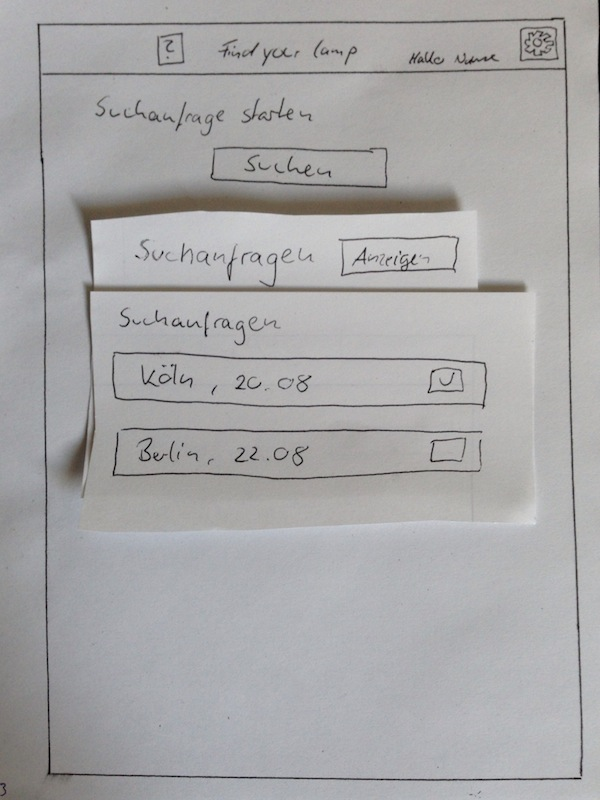
\includegraphics[width=.42\textwidth]{./images/paperbased//anfrage.JPG}}
\hfill %
\caption{Paperbased Prototype: Beispielhafte Interfacedarstellungen }
\label{proto}
\end{figure}

\subsection{Evaluation}
Nachdem sich der Prototyp durch interne Tests dadurch auszeichnete, einfache Anforderungen durchzuspielen zu können, sollte der erstmalige Einbezug realer Benutzer erfolgen.\\
Das Ergebnis der Benutzermodellierung stellte bereits heraus, dass sich potentielle Anwender nicht durch besondere Charakteristiken hervorheben lassen. Für eine möglichst effektive Bewertung, wäre an dieser Stelle der Einbezug von Leuten vorgesehen, die Interesse am Konzept der Anwendung haben und eventuell sogar Erfahrungen in der Domäne mitbringen. Solche Personen konnten für die Evaluation aber nicht gewonnen, sodass ein Rückgriff auf die Personae angedacht war. Ein Hindernis in dieser Hinsicht stellte dann die Diskussion dar, das eine Evaluation anhand der Personae weiterhin nur auf den eigenen Konzepten und Ideen beruhen würde.
Auch wenn sich ein Teammitglied in die Rolle hinein versetzen würde, so kann keine Auseinandersetzung aus der Sicht eines unvoreingenommenen Anwendern simuliert werden.
Daher wurde letztendlich auf Testpersonen zurückgegriffen, die sich mit Hilfe einer kurzen Einführung in die Thematik, in entsprechende Rolle hineindenken sollten.\\
Zuvor folgte die Auswahl einer geeigneten Evaluationsmethoden, anhand projektspezifischer Merkmale. 
Grundsätzlich sollte die Evaluationen einen empirischen Ansatz verfolgen und unter Einbezug von Stakeholdern durchgeführt werden. Ein analytischer Ansatz unter Einbezug von MCI Spezialisten kam aufgrund des Anforderungslevels nicht in Frage.
Der Zeitpunkt der Evaluation ist während der Entwicklungsphase, sodass eine formative Evaluationsart einer summativen vorgezogen wird. Die erhobenen Daten sollten in sprachbasierter Form vorliegen (qualitativ), da keine Messvorgänge und zahlenbasierte Ergebnisse das gewünschte Ziel verdeutlichen würden.\\
Zur Option standen weiterhin mehrere Techniken wie das Think aloud, Interviews, Umfragen oder die Beobachtung.
Da Umfragen aufgrund ihres psychologischen Charakters nur schwer umzusetzen sind, entfiel diese Methodik. Umfragen oder Beobachtung, erschienen für einen papierbasierten Prototypen nicht optimal und können durch Interpretation beeinflusst werden, aufgrund dess die Wahl auf die \textbf{Think aloud} Technik fiel.\\
Zu Beginn der Evaluation stand die Interaktionsphase, innerhalb derer mit den Probanden eine Einführung durchgeführt wurde. Die Ausgangsituation und das Vorgehen wurde erläutert und Informationen zum Tester und vorhandene Kenntnisse zur Domänenerfahrung wurden eingeholt.\\
Anschließend folgte die Durchführungsphase, bei der die Tester vor unterschiedliche Aufgaben gestellt wurden und während der Ausführung Gedanken äußern sollten. Nach erfolgreicher Durchführung folgte eine abschließende Besprechung mit Feedback zum Designansatz und weitere Aspekte, die sie sich für die Anwendung wünschen würden.\\
Ergebnisse wurden von einem Protokollanten erstellt, während der Zweite als Moderator durch die Evaluation führte.
Insgesamt wurden für diesen Prototypen 2 Tests durchgeführt, wobei die Ergebnisse des ersten Probanten im Evaluationsprotokoll Abb. \ref{fig:evaluation11} und Abb. \ref{fig:evaluation12} und die Ergebnisse des Zweiten im Protokoll in Abb. \ref{fig:evaluation21} und Abb. \ref{fig:evaluation22} dargestellt sind.

\newpage

\begin{figure}[H]
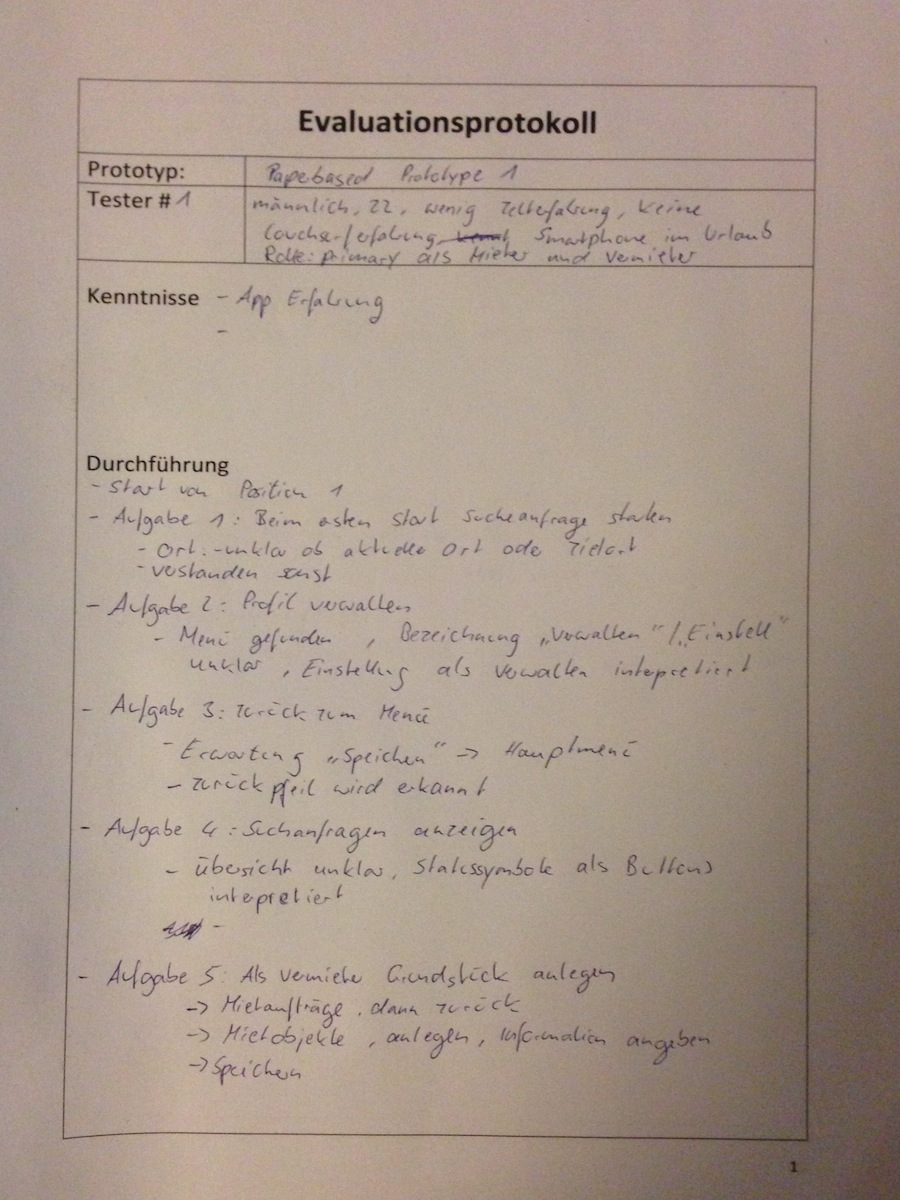
\includegraphics[width=1\textwidth]{./images/evaluation/eva11.JPG}
\caption{Evaluationsprotokoll 1.1}
\label{fig:evaluation11}
\end{figure}

\begin{figure}[H]
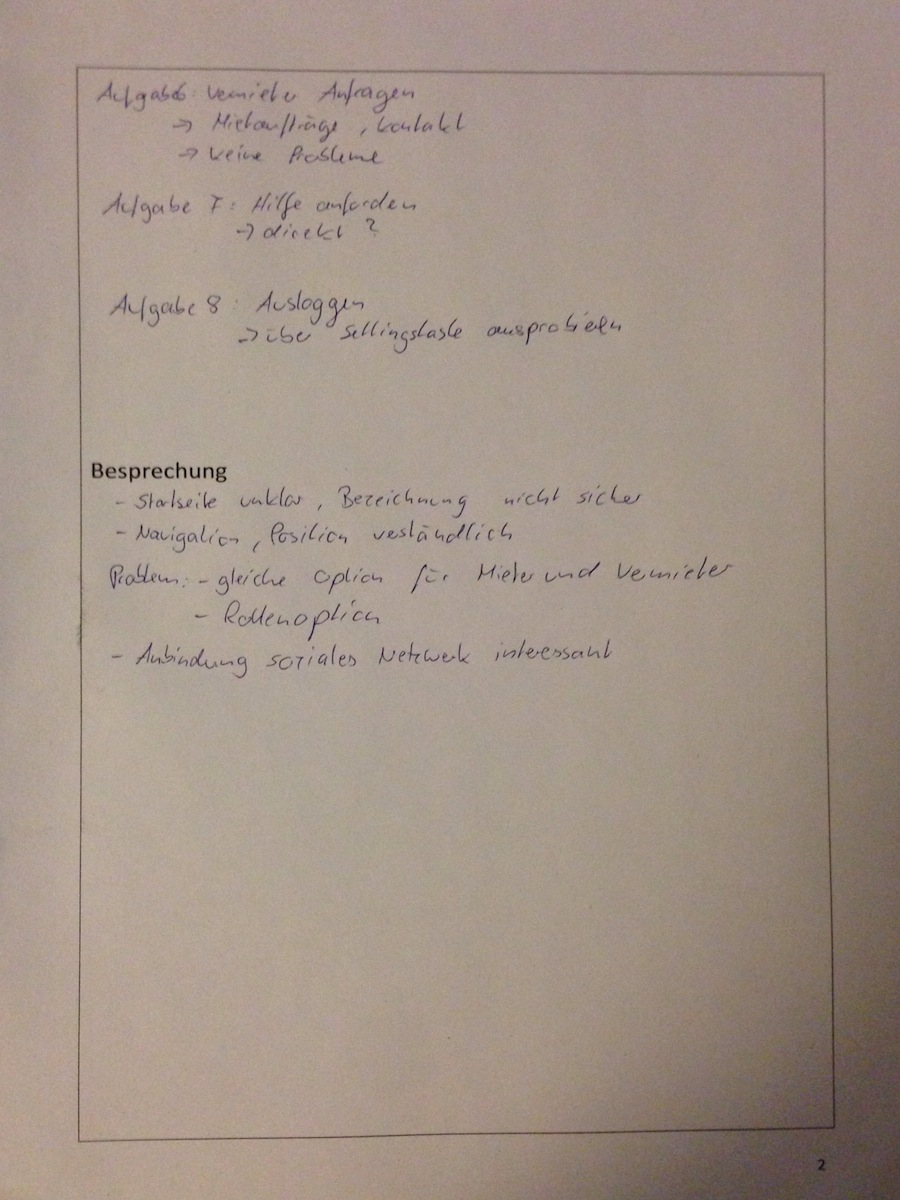
\includegraphics[width=1\textwidth]{./images/evaluation/eva12.JPG}
\caption{Evaluationsprotokoll 1.2}
\label{fig:evaluation12}
\end{figure}

\begin{figure}[H]
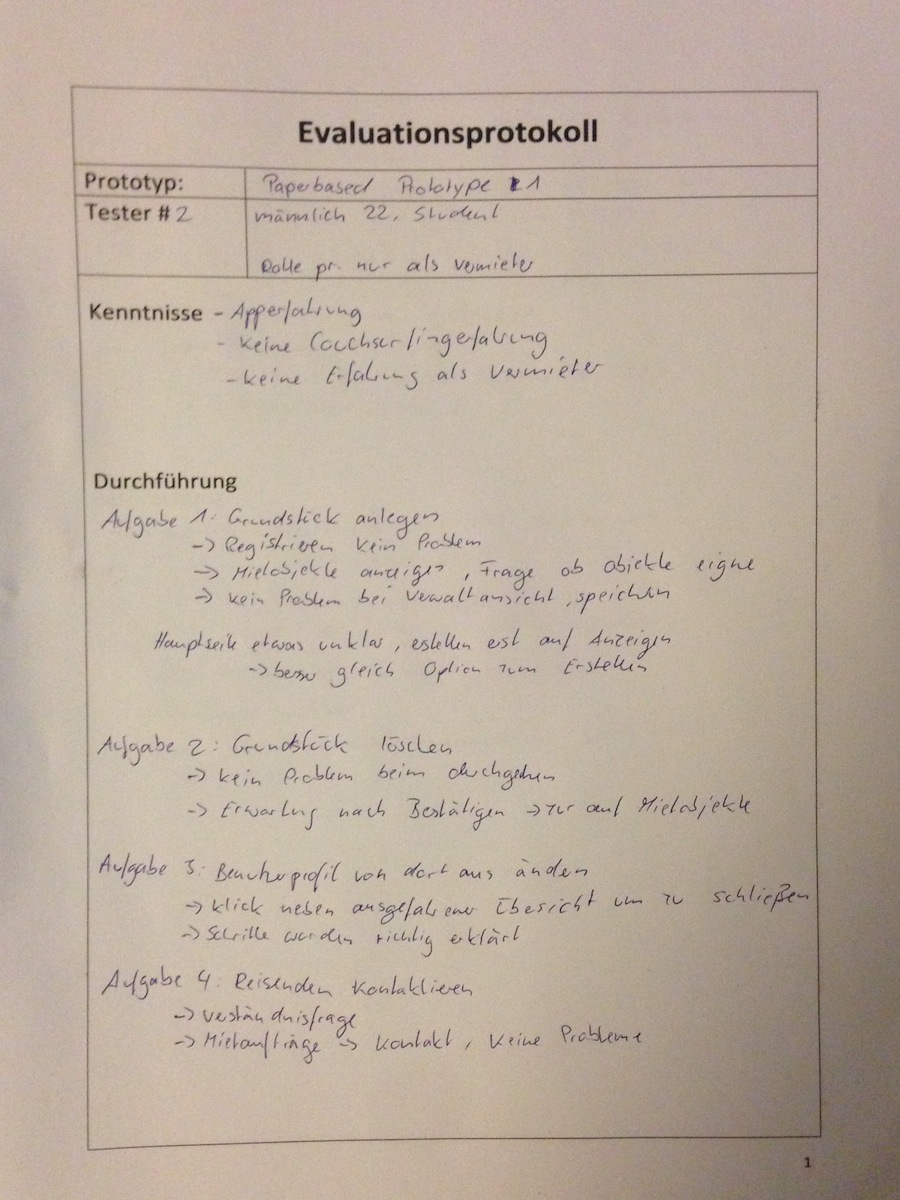
\includegraphics[width=1\textwidth]{./images/evaluation/eva21.JPG}
\caption{Evaluationsprotokoll 2.1}
\label{fig:evaluation21}
\end{figure}

\begin{figure}[H]
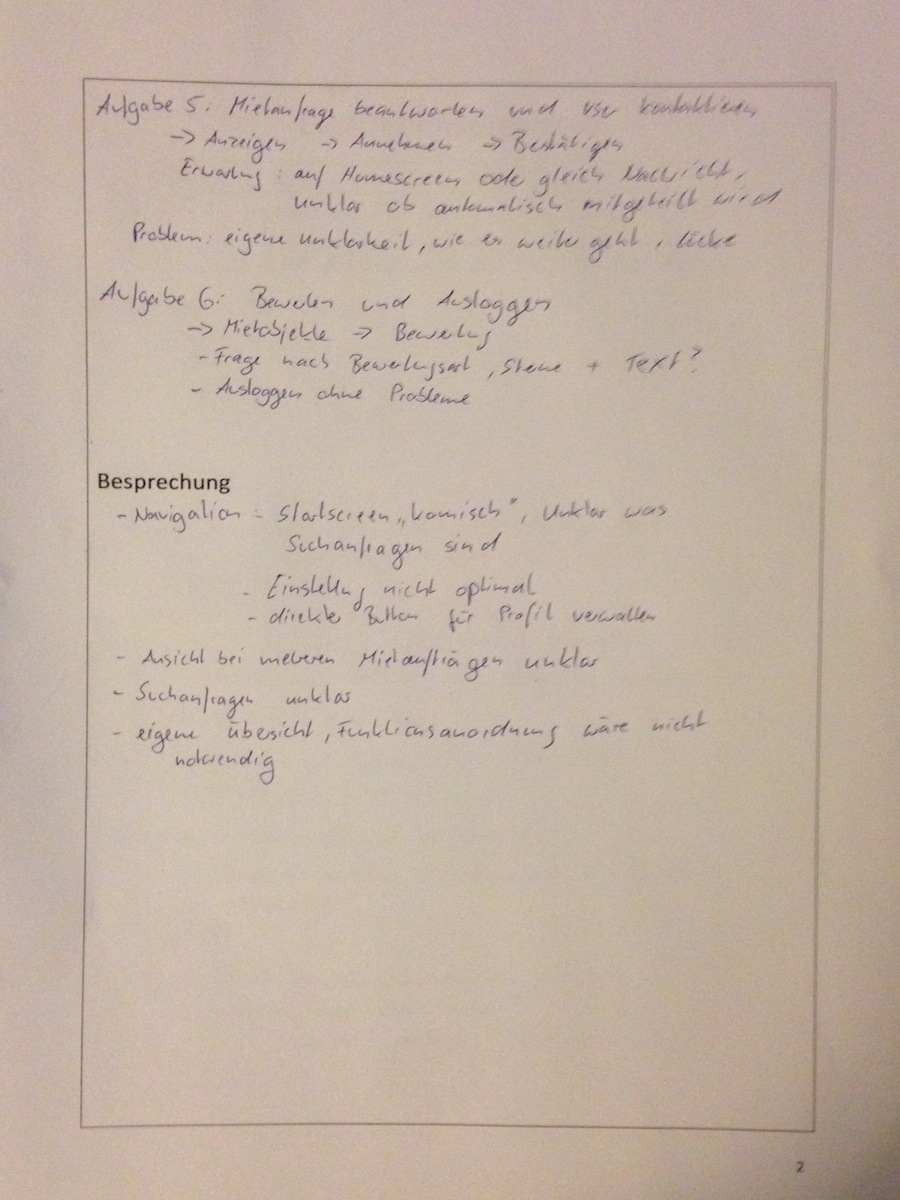
\includegraphics[width=1\textwidth]{./images/evaluation/eva22.JPG}
\caption{Evaluationsprotokoll 2.2}
\label{fig:evaluation22}
\end{figure}

\newpage
Im Anschluss wurden beide Evaluationen im Team diskutiert. Zusammenfassend lässt sich sagen, dass beide Testpersonen durch vorhandene Erfahrung mit Smartphones und Anwendungen, nach einer kurzen Eingewöhnungszeit keine Probleme hatten die Navigation zu verstehen und ein Verständnis dafür bekamen, wo sie sich strukturell befinden.
Unklarheiten traten durch ungünstige Formulierungen auf, da nicht immer eindeutig war, was mit den Bezeichnungen "Suchanfrage", "Mietobjekt" oder "Mietauftrag" gemeint ist. Eine Verbesserung in dieser Hinsicht soll durch eine genauere Bezeichnung erreicht werden.\\
Da die Benutzer sowohl in der Rolle des Mieters und Vermieters auftreten können, bot die erste Hauptseite (unnötiger Weise) die Funktionalitäten beider Rollen an. Auch das wurde angemerkt, da Anwender die nur in einer Rolle auftreten, somit überflüssige Informationen präsentiert bekommen. Das Problem hierbei bestand nicht unbedingt in der Komplexität dieses Interface, sondern vorallem an der Bezeichnung und der Struktur. Zusätzlich dazu, zeigten sich deutliche Schwächen in manchen Fenstern, wenn es um Übergänge zu den anderen Optionen ging. Besonders nach der Annahme einer Mietanfrage, war es sehr umständlich dem Reisenden eine direkte Nachricht zu senden. \\

\begin{wrapfigure}{r}{0cm}
\centering
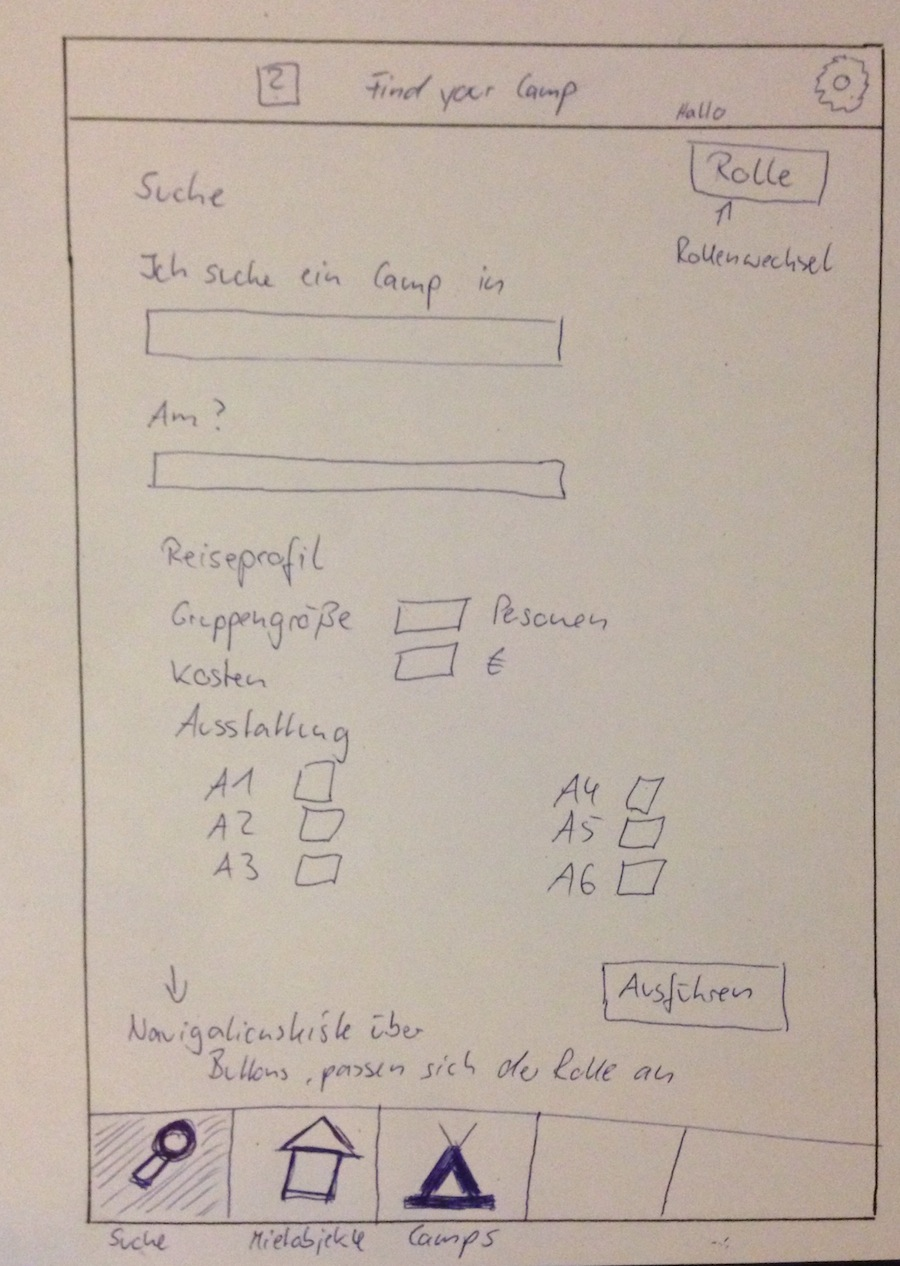
\includegraphics[width=.5\textwidth]{./images/mainneu.JPG}
\caption{PB Prototype 2: Überarbeitete Hauptseite }
\label{mainneu}
\end{wrapfigure}

Aufbauend darauf wurde eine überarbeitete Version des Prototypen entwickelt, bei dem vorallem die Hauptseite, dargestellt in Abb. \ref{mainneu}, von Grund auf neu angelegt wurde. Menübuttons werden hierbei mit Hilfe von Icons unter dem Ziel dargestellt, vorhandene Metaphern zu triggern. Eine tiefergehende Auseinandersetzung mit diesen mentalen Modellen, wurde im Projektverlauf herausgenommen, sollte jedoch als direkter Gegensatz zur textuellen Beschreibung in einer weiteren Evaluationsphase getestet werden. \\

 Die Gestaltung fand unter Einbezug der Grundsätze der Dialoggestaltung statt\footnote{Nach ISO 9241-110, in Prof. Hartmann Draftzur MCI ab S. 514}. Die Beschäftigung damit, war die letzte MCI Auseinandersetzung im Rahmen dieses Projektes und konnte bisher nur sehr oberflächlich betrachtet werden. \\

\newpage

\subsection{Grundsätze der Dialoggestaltung}
 ISO 9241 Teil 110
 Gestaltungsempfehlungen ISO Teil 12-17
\\
 1. Aufgabenangemessenheit\\
 	Fokus auf Aufgabe, nicht auf Technik\\
 	Dialogsystem: nur Informationen für Aufgabe, Hilfefunktion, \\automatische Ausführung, Eingabe Cursor im ersten Eingabe Widget, bei wiederkehrenden Aufgaben unterstützen = Speichern von aufeinander folgenden Interaktionsschritten, Standartwerte als Vorgabewerte\\
\\
 2. Selbstbeschreibungsfähigkeit\\
    Verständnis zum aktuellen Standpunkt im Dialog, was gemacht werden kann, wie man es ausführt\\
    Rückmeldung durch unmittelbares Anzeigen der Eingaben, bei schwerwiegenden Folgen Bestätigung einbauen, keine Fachterminologie, Begriffe erläutern und Benutzerhandbuch, Informationen zum aktuellen Stand, zB prozentualer Beabreitungsstand, Überblick über zukünftige Dialogschritte, Informationen zum Eingabedatentyp

 3. Steuerbarkeit\\
 	Geschwindigkeit unter der Kontrolle des Benutzers, Dialogsystem setzt immer auf nächsten Eingabecursor, sollte aber freie Interaktion ermöglichen. Interaktionsschritte sollten zurücknehmbar sein, auch auf das zurückgreifen zuvor gelöschter Objekte, Short Cuts?

 4. Erwartungskonformität\\
 	konsistent, Merkmalen der Benutzern entsprechend, Zustandsmeldungen immer an der selben Stelle, Interaktionssequenz wird immer durch selbe Taste beendet, ähnlichkeiten, Antwortzeiten mitteilen, zB über ladebalken, status widget, prozentsatz des datenvolumens

 5. Fehlertoleranz\\
 	testen des Datentypens nach Eingabe, Fehler erläutern mit Fehlermeldung, farbige hervorhebung 

 6. Individualisierbarkeit\\
 	Anpassung an individuelle Fähigkeit und Bedürfnisse, Schriftgröße und Farbe, Sprache

 7. Lernförderlichkeit\\
 	Fehlerbeschreibung, learning by doing durch hohe Fehlertoleranz, Übungsszenarien\\

 	in weiteren Iso nachschauen
 	das Erkennen und Spezifizieren von Dialoganforderungen auf der Grundlage der verschiedenen Dialogtechniken, die in den Teilen der Norm ISO 9241-14 bis ISO 9241-17 beschrieben sind;
 den Entwurf von Gestaltungslösungen unter Einhaltung von ISO 9241-12 bis ISO 9241-17\\


 



